\begin{figure}
  \centering
  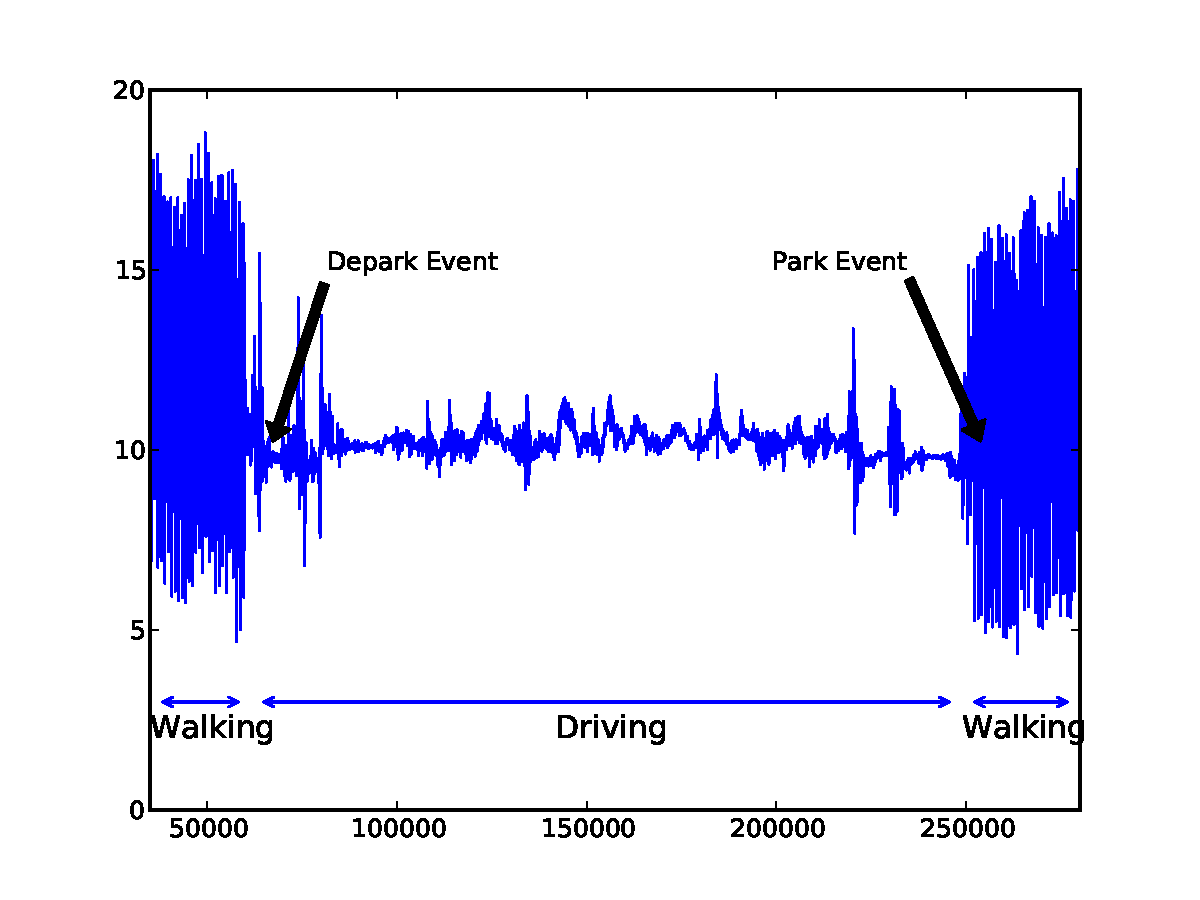
\includegraphics[scale=.45]{./figures/Detection.pdf}

  \caption{\textbf{Detection algorithm.} The graph shows data collected
    during our controlled experiment and shows a period of walking, followed by
    driving, followed by a return to walking. Transitions between these states
  indicate parking lot arrivals and departures.}

  \label{fig-detection}
\end{figure}

\section{Availability Estimation}
\label{sec-model}



\section{Event Detector}
\label{sec-detector}

The inputs to PocketParker's availability estimation algorithm are arrival and
departure events generated by an activity detector running unattended on users'
mobile devices.  While considerable previous research has explored activity
detection using mobile sensing~\cite{Constandache:2010:DYS, Keally:2011:PTP,
Reddy:2010:UMP, Yang:2011:DDP, Wang:2009:FEE}, we design a custom parking event
detector tailored to the goals of PocketParker.  In this section, we briefly
describe this detector and other portions of our system that run on the
smartphone itself.  

\subsection{Parking Events}
\label{subsec-goals}

PocketParker assumes that transitions between walking and driving that occur
in and adjacent to locations known to be parking lots constitute either
arrival (driving to walking) or departure (walking to driving) events.  We thus
must be able to discern between walking and driving states of the user, and to 
do so fast enough to fix the the location of the parking lot in which the
event took place.  Detecting these states could be achieved using
continuously-sampled GPS data would consume too much energy for an effective
pocketsourcing solution.  Rather, we rely on duty-cycled accelerometer data to
classify the user behavior into one of three states: walking, driving, or idle.

The initial inference of user states yielded by accelerometer sensing is
subsequently refined with GPS and WiFi sense data to yield the desired goal:
detection of arrival and departure events.  The mobile device reports these
events, along with their locations, to the server.  Before recording the event,
the server verifies its location against a pre-compiled list of known parking
lot locations.  This final step eliminates events that are either
incorrect (e.g., a user parking in a field) or unwanted (e.g., a user genuinely
parking but in a loading area rather than in a parking lot).

Subsequent to the conclusion of our research, Google released an update to its
closed Android binaries that contained user activity detection functionality.
As this was similar to that developed for PocketParker, substituting this
code would not have materially affected the detection of arrival and departure 
events.  Both algorithms treat user state detection in terms of relative
liklihoods.~\cite{recognition-confidence}  False detection could be further 
minimized with additional sensing, particularly GPS data, or with more 
computationally intense detection algorithms.  We have deliberately shied away 
from such an approach however, as the inherent nature of our application 
dictates that the bulk of testing and filtering takes place on an 
energy-constrained mobile platform.
